\clearpage
\section{Router-level topology}
\label{sec:router}

\subsection{A look back}
\label{sec:router_hist}

Since the early days of the ARPANET, networking researchers have been
interested in drawing the type of networks they
designed~\cite{heart78:_arpanet}.  An early map of the ARPANET is
reproduced in \autoref{fig:arpa_1971} and shows the network's logical
connectivity structures in April 1971, when the network as a whole
consisted of some 15 nodes and a node was little more than one or two
state-of-the-art computers connected via an Interface Message
Processor or IMP (the modern equivalent would be a router).  In this
context, logical structure refers to a detailed drawing of the
connectivity among those nodes and of node-specific details (\eg type
of machine), by and large ignoring geography.  In contrast, geographic
structure refers to a map of the US that includes the actual locations
of the network's physical nodes and shows the physical connectivity
among those nodes. Such accurate maps could be drawn because at that
time, each piece of equipment was expensive and needed to be accounted
for, only a few groups with a small number of researchers were
involved in the design and installation of the network, and the
network changed relatively slowly.

\begin{figure}[thbp]
  \begin{center}
    \begin{subfigure}[b]{0.75\textwidth} \centering
      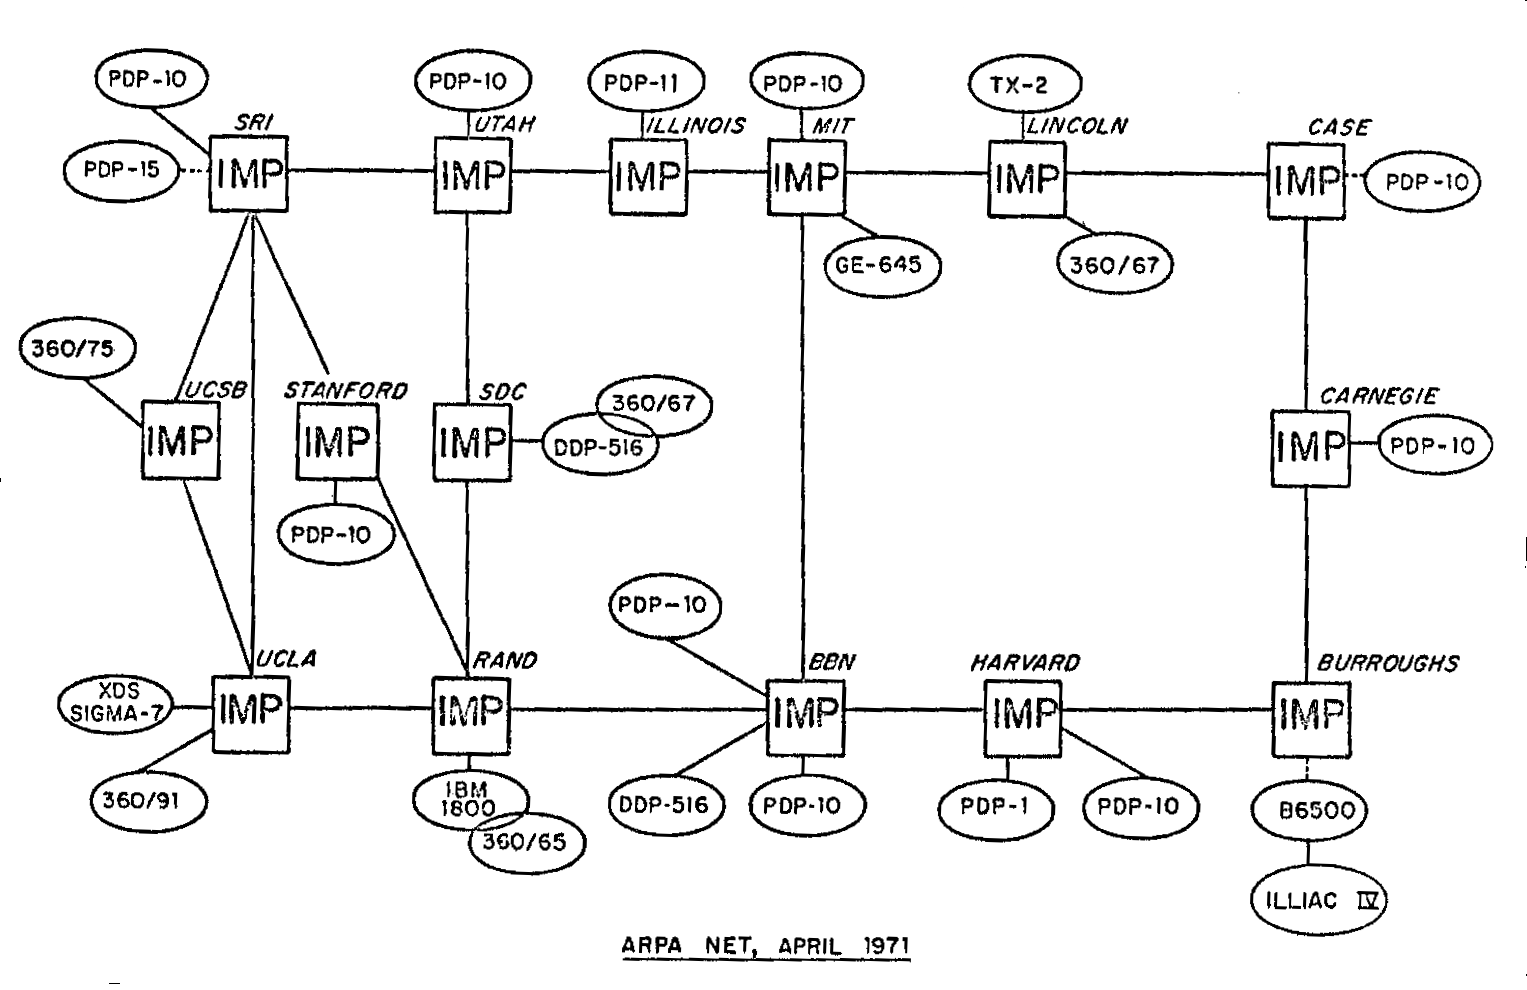
\includegraphics[width=1\textwidth]{cerf_arpanet_1971_april.png}
    \end{subfigure}
    \caption{The ARPANET in 1971 (reprinted from
      \cite{cerf90:_selected_maps}; \copyright 1990 ACM, Inc. Included here by permission.)
      \label{fig:arpa_1971}}
% \url{http://www.cs.utexas.edu/users/chris/DIGITAL_ARCHIVE/ARPANET/DARPA4799.pdf}
% (page III-144, page III-81)
  \end{center}
\end{figure}


\begin{figure}[thbp]
  \begin{center}
    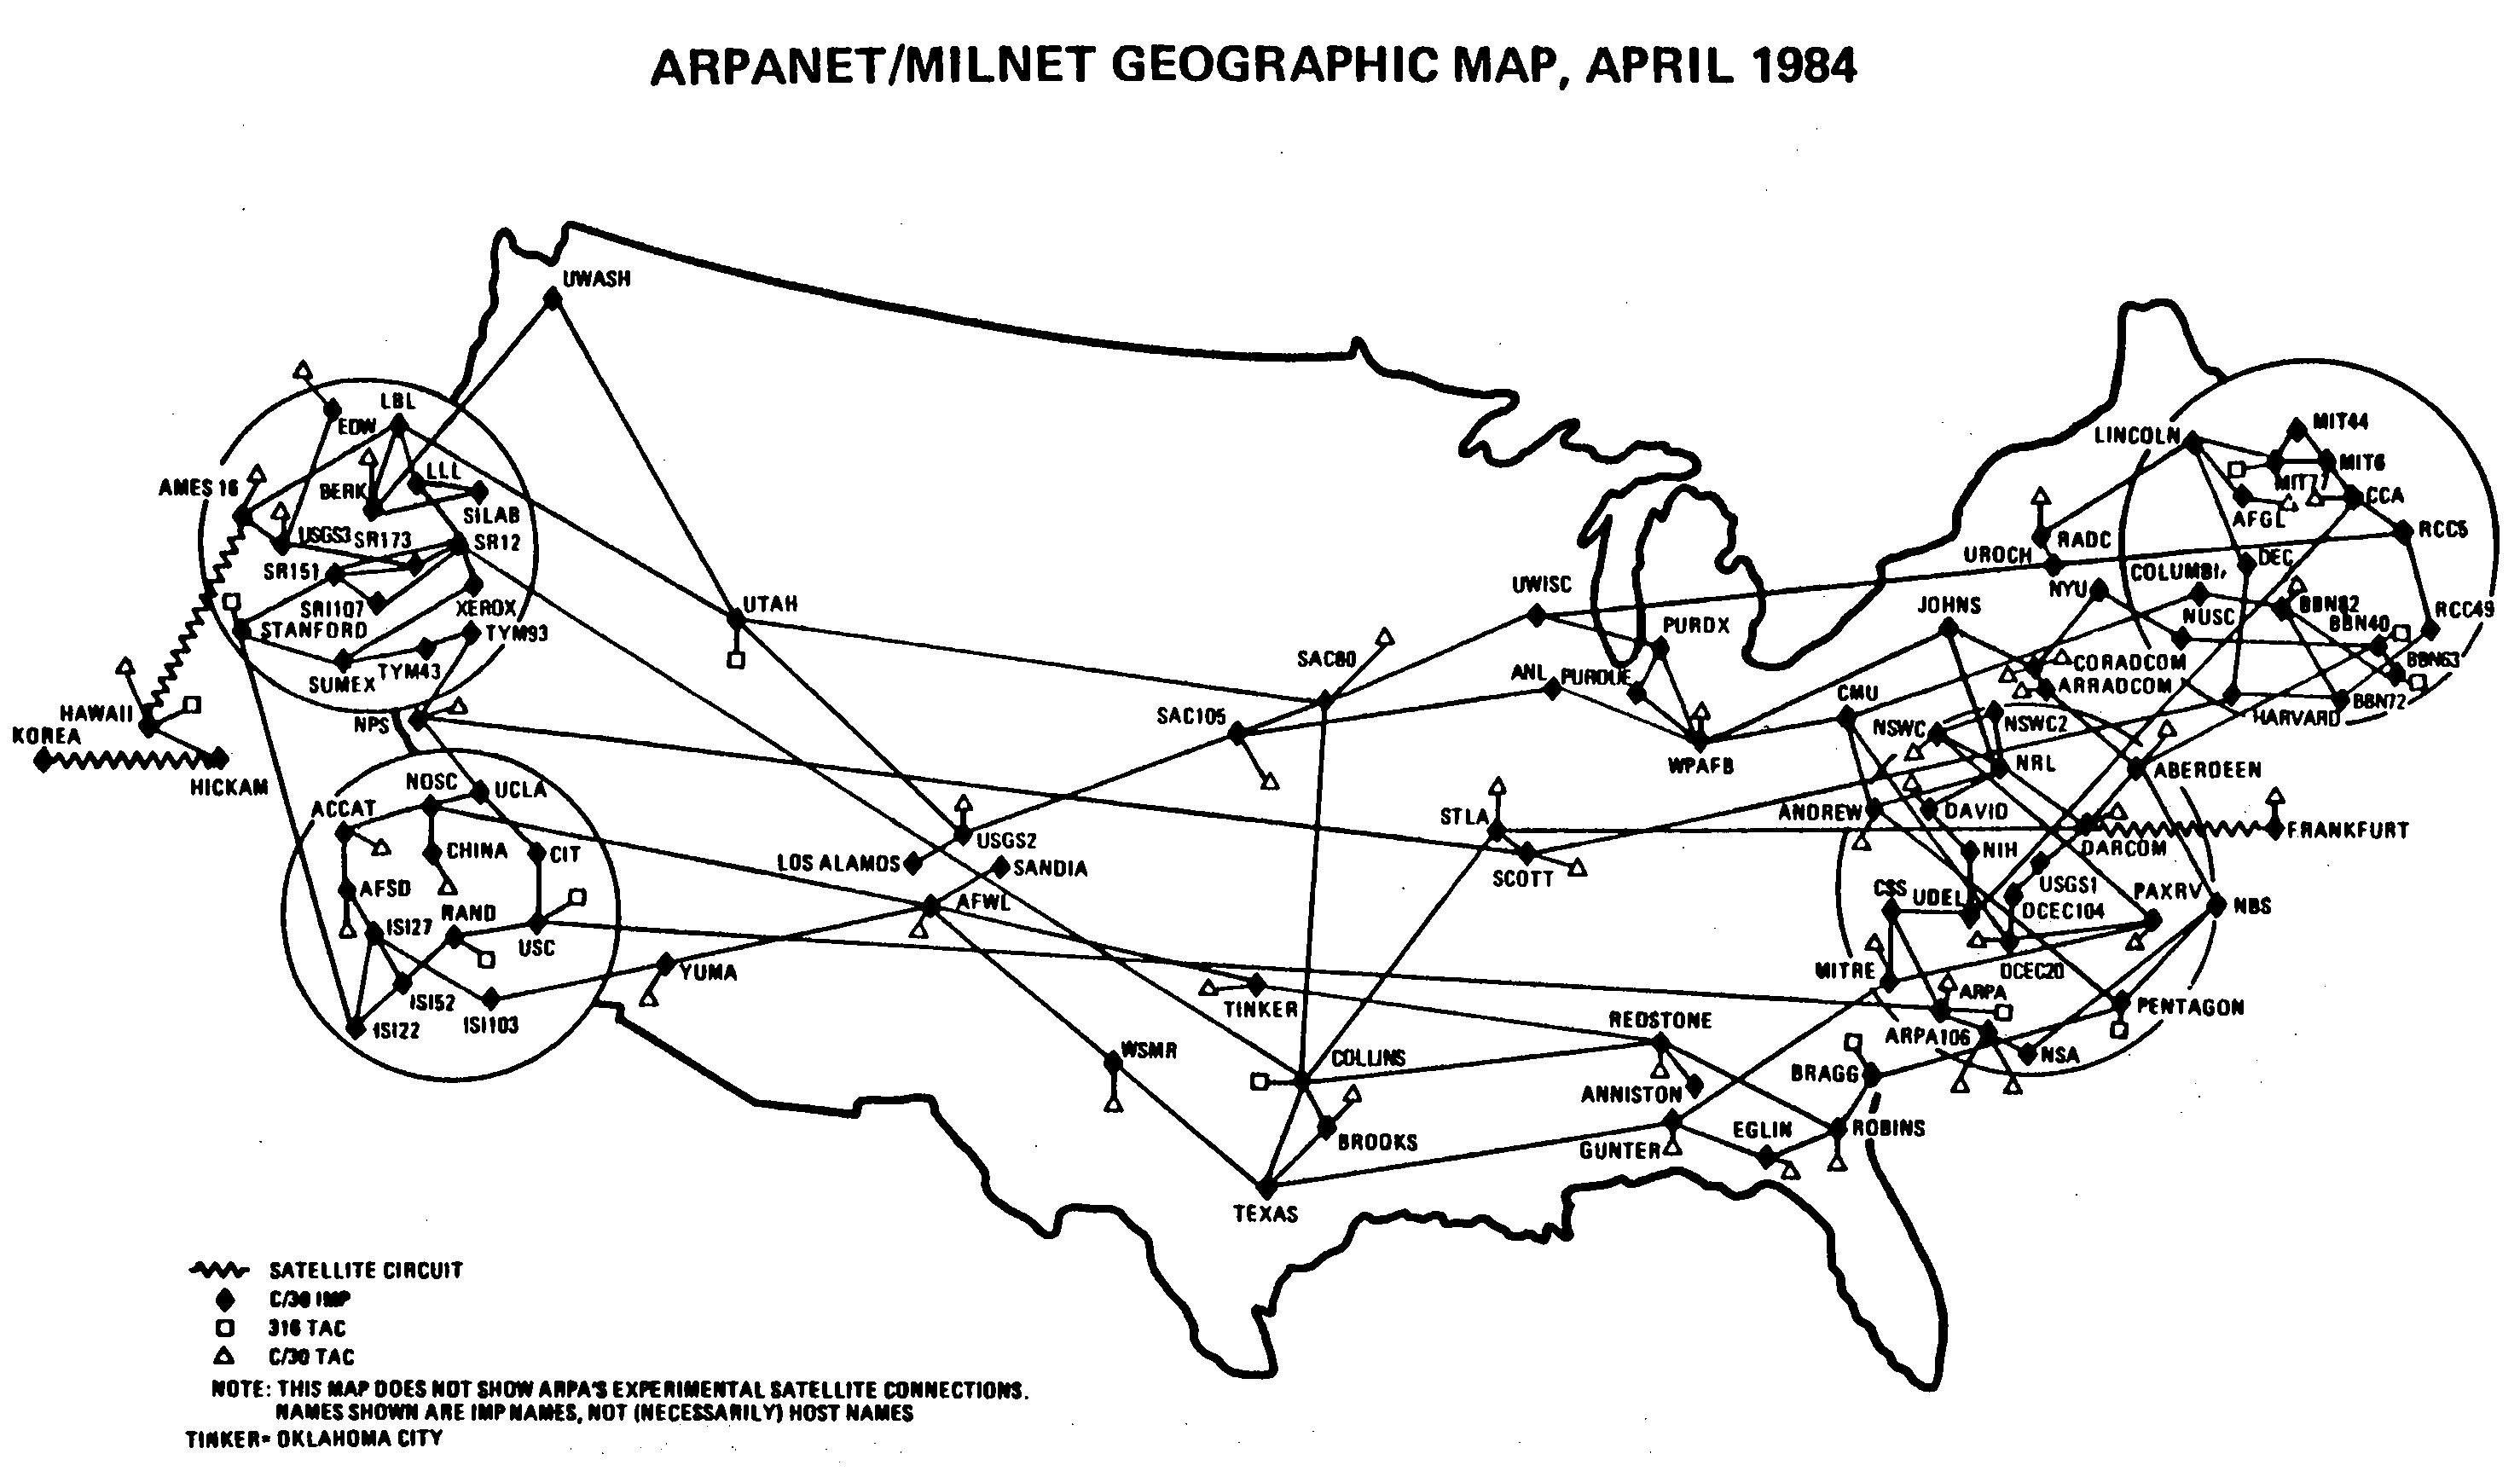
\includegraphics[width=0.9\textwidth]{cerf_arpanet_1984.png}
    \caption{The early ARPANET  (reprinted from
      \cite{cerf90:_selected_maps}; \copyright 1990 ACM, Inc. Included here by permission.)
      \label{fig:arpa_1984}}
  \end{center}
\end{figure}

The network quickly grew in size and complexity. For instance,
\autoref{fig:arpa_1984} shows the geographic counterpart from 1984 of
the ARPANET map depicted in \autoref{fig:arpa_1971}.  Manually
accounting for the increasing number of components quickly became
prohibitive and motivated the adoption of automatic strategies for
obtaining some of the available connectivity as well as traffic
information.  A prime example for effectively visualizing this
collected information is reproduced from
\cite{frazer:_merit_histor_nsfnet_backb_projec} and shown in
\autoref{fig:nsfnet}, which depicts a 3D rendering of the (US portion
of the) NSFNET around 1991, annotated with traffic-related
information. At that time, the NSFNET backbone consisted of some 14
nodes that were interconnected with T1 links as shown and, in turn,
connected to a number of different campus networks (\eg collections of
interconnected LANs). However, even though the internal structure of
the backbone nodes was well-known (\ie each node was composed of nine
IBM RTs linked by two token rings with an Ethernet interface to
attached networks), nobody had any longer access to the internals of
all the different campus networks and as a result, drawing the 1991
NSFNET equivalent of the ARPANET's logical connectivity structure
(\autoref{fig:arpa_1971}) was no longer possible.
 
\begin{figure}[thbp]
  \begin{center}
    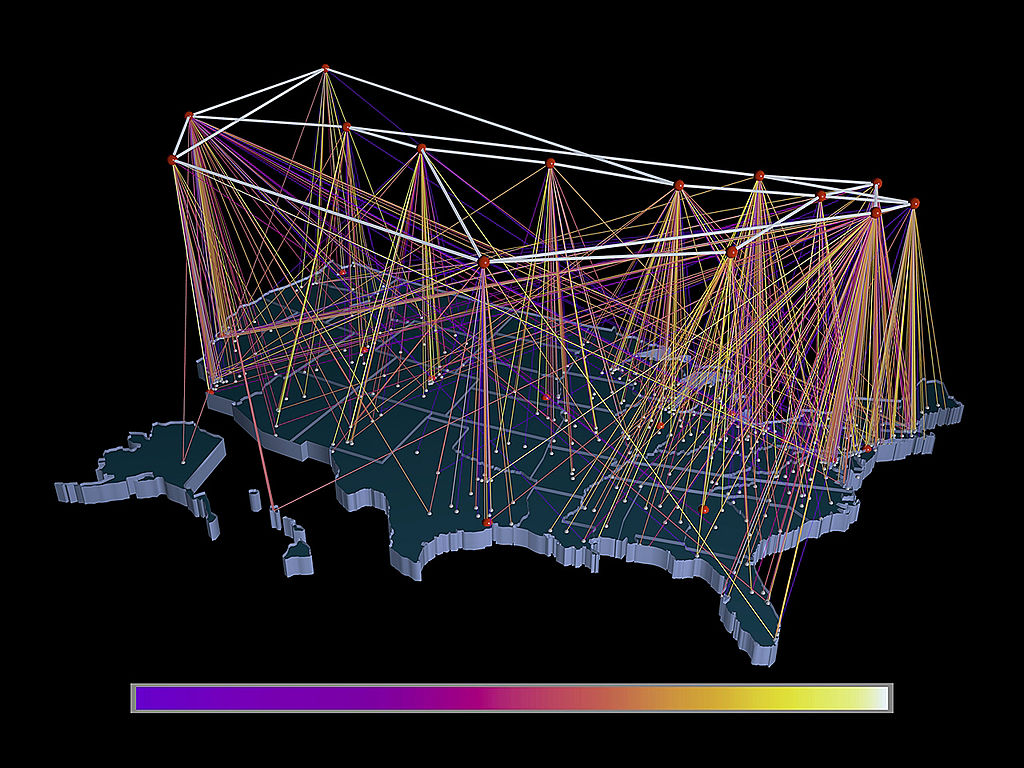
\includegraphics[width=0.7\textwidth]{1024px-NSFNET-traffic-visualization-1991.jpg}
    \caption{A visualization of the NSFNET circa 1991 (by Donna Cox
and Robert Patterson,
\href{http://avl.ncsa.illinois.edu/project-archive/visualizing-the-early-internet}{National
Center for Supercomputing Applications, University of Illinois at
Urbana-Champaign}. See also
\url{http://en.wikipedia.org/wiki/File:NSFNET-traffic-visualization-1991.jpg}).
      \label{fig:nsfnet}}
  \end{center}
\end{figure}

With the decommissioning of the NSFNET in 1995 and the rise of the
"public Internet", the researchers' ability to obtain detailed
connectivity and component information about the internals of the
different networks that formed the emerging "network of networks"
further diminished and generated renewed interest in the development of
abstract, yet informed, models for router-topology evaluation and
generation. For example, the Waxman model \cite{Waxman88}, a variation
of the classical Erd\"{o}s-R\'{e}nyi random graph model \cite{erdos60}
was the first popular topology generator commonly-used for network
simulation studies at the router level. However, it was largely
abandoned in the late 1990s in favor of models that attempted to
explicitly account for non-random structure as part of the network
design. The arguments that favored structure over randomness were
largely empirical in nature and reflected the fact that the inspection
of real-world router-level ISP networks showed clear signs of
non-random structures in the form of the presence of backbones, the
appearance of hierarchical designs, and the importance of locality.
These arguments also favored the notion that a topology generator
should reflect the design principles in common use; \eg to achieve
some desired performance objectives, the physical networks must
satisfy certain connectivity and redundancy requirements, properties
which are generally not guaranteed in random network topologies.
These principles were, for example, advanced in
\cite{Zegura96,Calvert97,Zegura97} and were ultimately integrated into
the popular Georgia Tech Internetwork Topology Models (GT-ITM)
\cite{gt_itm}.
 
These more structure-oriented router topology generators were viewed
as the state-of-the-art until around 2000 when, in turn, they were
largely abandoned in favor of a new class of random graph models whose
trademark was the ability to reproduce the newly discovered power-law
relationship in the observed connectivity (\ie node degree) of
router-level graphs of the Internet. This discovery was originally
reported in the seminal paper by
Faloutsos~\etal~\cite{faloutsos99:_power_law_relat_of_inter_topol},
who used a router-level graph constructed from data that was collected
a few years earlier by Pansiot and Grad~\cite{pansiot98:_inter} for
the purpose of obtaining some experimental data on the actual shape of
multicast trees in the Internet. The Boston university Representative
Internet Topology gEnerator (BRITE) \cite{Medina01} became a popular
representative of this new class of models, in part also because it
combined the more structure-oriented perspective of the GT-ITM
generator with the new focus that emphasized the ability to reproduce
certain metrics or statistics of measured router topologies (\eg node
degree distribution).

One of the hallmarks of networks that have power-law degree
distributions and that are generated according to any of a number of
different probabilistic mechanisms (\eg preferential attachment
\cite{barabasi99}, random graphs with a given expected degree sequence
\cite{Chung04}, power-law random graphs 
\cite{Aiello00}) is that they can be shown to have
a few centrally located and highly connected {\em hubs} through which
essentially most traffic must flow.  When using these models to
represent the router-level topology of the Internet, the presence of
these highly connected central nodes has been touted the Internet's
``Achilles-heel'' because network connectivity is highly vulnerable to
attacks that target the high-degree hub nodes \cite{barabasi00}. It has been
similarly argued that these high-degree hubs are a primary reason for
the epidemic spread of computer worms and viruses \cite{berger05:_spread_of_viruses,pastor-satorras01:_epidem}.
Importantly, the presence of highly connected central nodes in a
network having a power-law degree distribution is the essence of the
so-called scale-free network models. They have been a highly popular
theme in the study of complex networks, particularly among researchers
inspired by statistical physics \cite{albert_barabasi02}, and have fuelled the rise of
a new scientific discipline that has become known as ``Network
Science" \cite{barabasi12}.  In the process, they have also seen wide-spread
use among Internet topology researchers.

However, as the general fascination with and popularity of network
science in general and scale free network modeling in particular grew,
so did the arguments that were voiced by Internet researchers
and questioned the appropriateness and relevance of the scale-free
modeling approach for studying highly-engineered systems such as the
Internet's router topology. In fact, at around 2010, when the number
of publications in the area of network science reached a new height,
the number of papers that were published in the networking research
literature and applied scale-free network models to describe or study
router-level topologies of the Internet was close to zero.  This begs
the question ``What happened?'', and the answer provided in the next
section is really a classic lesson in how errors of various forms
occur and can add up to produce results and claims that create
excitement among non-networking researchers, but quickly collapse when
scrutinized with real data or examined by domain experts.



\subsection{Know your measurements}
\label{sec:router_measurements}

Between 1990 and 2000, Internet topology research underwent a drastic change from being
a data-starved discipline to becoming a prime example of a largely measurement-driven research 
activity.  As described earlier, even though the development of abstract, yet informed,
models for network topology evaluation and generation has always been a give and take between
theoreticians and empiricists, for router topology modeling, the essential role that
measurements have started to play came into full focus in a sequence of three seminal papers that
appeared between 1998-2000. 

\subsubsection{Three seminal papers on router topology modeling}
\label{sec:router_seminal}

The key papers that turned router topology modeling into a full-fledged measurement-driven
research activity cover the whole spectrum of modeling activities, from
measurement experiments to model construction and validation to graph-theoretical network
analysis, and are listed below: 

\begin{itemize}
\item[(i)] ``On routes and multicast trees in the Internet'' by
  J.-J. Pansiot and D. Grad (1998) \cite{pansiot98:_inter} described
  the original measurement experiment that was performed in mid-1995
  and produced data on actual routes taken by packets in the
  Internet. This data was subsequently used to construct a router
  graph of the Internet.

\item[(ii)] ``On power-law relationships of the Internet topology'' by
  M. Faloutsos~\etal~(1999)
  \cite{faloutsos99:_power_law_relat_of_inter_topol} reported (among
  other observations) on the observed power-law relationship in the
  connectivity of the router-level topology of the Internet measured
  by Pansiot and Grad~\cite{pansiot98:_inter}.

\item[(iii)] ``Error and attack tolerance of complex networks'' by
  R. Albert~\etal~(2000) \cite{barabasi00} proposed a scale-free
  network model to describe the router topology of the Internet and
  argued for its validity on the basis of the latest findings by
  Faloutsos~\etal~\cite{faloutsos99:_power_law_relat_of_inter_topol}.
  It touted the new model's exemplary predictive power by reporting on
  the discovery of a fundamental weakness of the Internet (a property
  that was became known as the Internet's "Achilles' heel") that went
  apparently unnoticed by the engineers and researchers who have
  designed, deployed, and studied this large-scale, critical
  infrastructure, but followed directly from the newly proposed
  scale-free modeling approach.
\end{itemize}

\begin{figure}[!htp] 
  \begin{center}
    \includegraphics*[width=0.8\columnwidth,viewport=0mm 52mm 260mm 160mm]{ams-figs-final.pdf}
    \caption{A toy example of a scale-free network of the preferential
      attachment type (b) generated to match a power-law type node
      degree distribution (a).  (First published in Notices of the
      American Mathematical Society, Volume 56, No.3 (May 2009):
      586-599 \cite{willinger09:_mathem_and_inter}. Included here by
      permission.)
      \label{fig:hot_1}}
    % \url{http://www.ams.org/notices/200905/rtx090500586p.pdf}  (figure 1)
  \end{center}
\end{figure}         


At first glance, the combination of these three papers appears to show
network modeling at its best -- firmly based on experimental data,
following modeling practices steeped in tradition, and discovering
surprisingly and previously unknown properties of the modeled network.
An example of a toy network resulting from taking the findings from
these seminal papers at face value is shown in \autoref{fig:hot_1}.
However, one of the beauties of studying man-made systems such as the
Internet is that -- because of their highly-engineered architectures,
a thorough understanding of its component technologies, and the
availability of extensive (but not necessarily very accurate)
measurement capabilities -- they provide a unique setting in which
most claims about their properties, structure, and functionality can
be unambiguously resolved, though perhaps not without substantial
efforts. In the remainder of this section, we will illustrate how in
the context of the Internet's router topology, applying readily
available domain knowledge in the form of original design principles,
existing technological constraints, and available measurement
methodologies reveals a drastically different picture from that
painted in these three seminal papers. In fact, we will expose the
specious nature of scale-free network models that may appeal to more
mathematically inclined researchers because of their simplicity or
generality, but besides having no bearing on the Internet's router
topology are also resulting in wrong claims about the Internet as a
whole.


\subsubsection{A first sanity check: Using publicly available information}



A first indication of apparent inconsistencies between the proposed
scale-free models for the Internet's router topology and the actual
Internet comes from the inspection of the router topologies of actual
networks that make the details of their network internals publicly
available. For example, networks such as Internet2~\cite{internet2} or
G\'{E}ANT~\cite{geant} show no evidence that there exist any centrally
located and highly connected ``hubs'' through which essentially most
traffic must flow.  Instead, what they typically show is the presence
of a more or less pronounced ``backbone'' network that is fed by
tree-like access networks, with additional connections at various
places to provide a degree of redundancy and robustness to components
failures\footnote{This is not a universal phenomena. For instance
  \cite{Zoo} notes that some networks do exhibit hub-like structure, but
  it is the lack of universality that is important here, as exhibited
  by these and other counter examples.}.

This design pattern is fully consistent with even just a cursory
reading of the most recent product catalogs or white papers published
by the main router vendors
\cite{cisco13:_build_cost_effec_scalab_core,cisco13:_converged,juniper13:_evolv_backb_networ_using_mpls_super}.
For one, the most expensive and fastest or highest-capacity pieces of
equipment are explicitly marketed as backbone routers. Moreover, due
to inherent technological limitations in how many packets or bytes a
router can handle in a given time interval, even the latest models of
backbone routers can support only a small number of very
high-bandwidth connections, typically to connect to other backbone
routers. At the same time, a wide range of cheaper, slower or
lower-capacity products are offered by the different router vendors
and are targeted primarily at to support network access.  On the
access side, a typical router will have many lower-bandwidth
connections for the purpose of aggregating customer traffic from the
network's edge and subsequently forwarding that traffic towards the
backbone. In short, even the latest models advertised by today's
router vendors are limited by existing technologies, and even for the
top-of-the-line backbone routers, it is technologically infeasible to
have hundreds or thousands of high-bandwidth connections. At the same
time, while technically feasible, deploying some of the most expensive
equipment and configuring it to support hundreds or thousands of
low-bandwidth connections would be considered an overall bad
engineering decision (\eg excessively costly, highly inefficient, and
causing serious bottlenecks in the network).
 
However, the root cause for these outward signs of a clear mismatch
between the modeled and actual
router topology of the Internet goes deeper and lies in the original design philosophy of the
Internet.  As detailed in \cite{clarke95:_design}, while the top level goal for the original DARPA Internet architecture was {\it ``to develop an effective technique for multiplexed utilization
of existing interconnected networks"}, the requirement that {\it ``Internet communication must
continue despite loss of networks or gateways"} topped the list of second level goals. To survive
in the face of components failing off, the architecture was to mask completely any transient 
failure, and to achieve this goal, state information which describes an existing connection must
be protected. To this end, the architecture adopted the ``fate-sharing" model that gathers this 
state information at the endpoints of connections, at the entities that are utilizing the 
service of the network. Under this model, it is acceptable to lose the state information 
associated with an entity if, at the same time, the entity itself is lost; that is, there 
exists no longer any physical path over which any sort of communication with that entity can
be achieved (\ie total partition). Ironically, these original design principles
outlined in \cite{clarke95:_design} favor precisely the opposite of what the scale-free modeling approach
yields -- no centrally located and highly connected ``hubs'' because their removal makes
partitioning the network easy.


\subsubsection{An in-depth look at traceroute: \\ Examining a popular measurement technique}
\label{sec:mpls}

While the above-mentioned empirical, technological, and architectural
arguments cast some serious doubts on the scale-free network modeling
approach for the router topology of the Internet, they say nothing
about the measurements that form the basis of this approach and has
given it a sense of legitimacy among scientists in general and
networking researchers in particular.  To appreciate the full role
that measurements play in this discussion, it is informative to
revisit the original paper by Pansiot and Grad~\cite{pansiot98:_inter}
that describes the measurement experiment, discusses the measurement
technique used, and provides a detailed account of the quality of the
data that form the basis of the scale-free approach towards modeling
the Internet's router topology.

In essence, \cite{pansiot98:_inter} describes the first (at that time)
large-scale traceroute campaign performed for the main purpose of
constructing a router graph of the Internet from actual Internet
routes. Although traceroute-based, the authors of
\cite{pansiot98:_inter} quickly point out that their purpose of using
the traceroute tool (\ie obtaining actual Internet routes to
construct a router graph) differed from what V. Jacobson
\cite{jacobson89:_tracer} had in mind when he originally designed the
tool (\ie tracing a route from a source to a destination for
diagnostic purposes).  As a result, a number of serious issues arise
that highlight why using the traceroute technique for the purpose of
constructing a router graph is little more than an "engineering hack"
and can certainly not be called a well-understood "measurement
methodology."

{\bf IP alias resolution problem:} One serious problem
explained in detail in \cite{pansiot98:_inter} with using traceroute-based data for
constructing router graphs is that the traceroute tool only returns
the IP addresses of the interface cards of the routers that the probe
packets encountered on their route from the source to their
destination.  However, most routers have many interface cards, and
despite many years of research efforts that have produced a series of
increasingly sophisticated heuristics \cite{bender08:_fixin_allys,gunes09:_resol_ip_inter,sherry10:_resol_ip_alias_presp_times}, the networking
community still lacks rigorous and accurate methods for resolving the
IP alias resolution problem; that is, determining whether two
different interface IP addresses belong to or can be mapped to the
same router. While the essence of this problem is illustrated in
\autoref{fig:hot_2}, the impact it can have when trying to map a
router topology of an actual network is shown in \autoref{fig:hot_3}.


\begin{figure}[!htp] 
  \begin{center}
% pdfimages gets actual 'images' (bitmaps) out of the PDF, but not plots
% pdfjam ams-figs-final.pdf '5' --outfile ams-figs-p5.pdf
%     extracts a particular page so I can use it here
    \includegraphics*[width=0.6\columnwidth,viewport=10mm 110mm 200mm 200mm]{ams-figs-p2.pdf}
%                                                    xleft ybottom xright ytop
%                                                 a4 = 0 0 210 297
    \caption{The IP alias resolution problem. Paraphrasing Fig. 4 of \cite{rocketfuel_1}, 
	 traceroute does not list routers (boxes) along paths but IP addresses of 
	 input interfaces (circles), and alias resolution refers to the correct 
	 mapping of interfaces to routers to reveal the actual topology. In the case
	 where interfaces 1 and 2 are aliases, (b) depicts the actual topology while 
	 (a) yields an ``inflated'' topology with more routers and links.
	 (First published in Notices of the American Mathematical Society, Volume 56, 
	 No.3 (May 2009): 586-599 \cite{willinger09:_mathem_and_inter}. Included here by permission.)
      % \cite[Figure~2]{willinger09:_mathem_and_inter}.
      \label{fig:hot_2}}
    % \url{http://www.ams.org/notices/200905/rtx090500586p.pdf}  (figure 2)
  \end{center}
\end{figure}         

\begin{figure}[thbp] 
  \begin{center}
% pdfimages gets actual 'images' (bitmaps) out of the PDF, but not plots
% pdfjam ams-figs-final.pdf '5' --outfile ams-figs-p5.pdf
%     extracts a particular page so I can use it here
    \includegraphics*[width=1\columnwidth,viewport=0mm 70mm 210mm 240mm]{ams-figs-p3.pdf}
%                                                    xleft ybottom xright ytop
%                                                 a4 = 0 0 210 297
    \caption{The IP alias resolution problem in practice. Shown is a comparison 
	 between the Abilene/Internet2 topology inferred by Rocketfuel (left) and the 
	 actual topology (top right). Rectangles represent routers with interior ovals 
	 denoting interfaces. The histograms of the corresponding node degrees are 
	 shown in the bottom right plot. 
	 (Reprinted from \cite{sherwood08:_discar}; \copyright 2008
         ACM. Inc. Included here by permission.)
         \label{fig:hot_3}}
    % \url{http://www.ams.org/notices/200905/rtx090500586p.pdf}  (figure 3)
  \end{center}
\end{figure}         

\clearpage
{\bf Lesson 1:} {\em Due to the absence of accurate and rigorous methods for solving the IP alias
resolution problem, the actual values of the connectivity of each router (\ie node degrees)
inferred from traceroute measurements cannot be taken at face
value.}

{\bf Opaque Layer-2 clouds:} Another serious issue with
using generic traceroute-based measurements for construction router
graphs is also discussed at length in \cite{pansiot98:_inter} and
illustrated in \autoref{fig:hot_4}.  Being strictly limited to IP or
layer-3, the problem with traceroute is that it is incapable of
tracing through opaque layer-2 clouds that feature circuit
technologies such as Asynchronous Transfer Mode (ATM) or Multiprotocol
Label Switching (MPLS). These technologies have the explicit and
intended purpose of hiding the network's physical infrastructure from
IP, so from the perspective of traceroute, a network that runs these
technologies will appear to provide direct connectivity between
routers that are separated by local, regional, national, or even
global physical network infrastructures. An example of using
traceroute to map a network that uses MPLS is depicted in
\autoref{fig:hot_4} and shows an essentially completely connected
graph at Layer 3 with multiple high-degree nodes, even though the
physical router topology is very sparse. Similarly, if traceroute
encounters an ATM cloud, it falsely ``discovers'' a high-degree node
that is really a logical entity -- often an entire network potentially
spanning many hosts or great distances -- rather than a physical node
of the Internet's router-level
topology. Donnet~\etal~\cite{benoit12:_reveal_mpls} found that at
least 30\% of the paths they tested traversed an MPLS tunnel.

Recent extensions of the ICMP protocol, using traceroute to trace
through opaque MPLS clouds have become technically
feasible~\cite{rfc4950}, but operators often configure their routers to
hide the MPLS tunnels by turning off this option
\cite{sommers11:_preval_charac_mpls_deploy_open_inter}. Even then it
may be possible to detect the MPLS tunnels
\cite{benoit12:_reveal_mpls}, but the inference techniques are not a
guarantee, and are quite particular to MPLS, which is not the only
technique for creating tunnels, so there may still be some opaque
networks to deal with.  More to the point, even where such inferences
are possible, most data sets do not contain this type of analysis, and
most subsequent analyses of the data have ignored the issue.


\begin{figure}[thbp] 
  \begin{center}
% pdfimages gets actual 'images' (bitmaps) out of the PDF, but not plots
% pdfjam ams-figs-final.pdf '5' --outfile ams-figs-p5.pdf
%     extracts a particular page so I can use it here
    \includegraphics*[width=1\columnwidth,viewport=17mm 70mm 193mm 240mm]{ams-figs-p4.pdf}
%                                                    xleft ybottom xright ytop
%                                                 a4 = 0 0 210 297
    \caption{How traceroute detects fictitious high-degree nodes in
      the network core. (a) The actual connectivity of an opaque
      layer-2 cloud, i.e., a router-level network running a technology
      such as ATM or MPLS (left) and the connectivity inferred by
      traceroute probes entering the network at the marked router
      (right).  (b) The Rocketfuel-inferred backbone topology of
      AS3356 (Level3), a Tier-1 Internet service provider and leader
      in the deployment of MPLS.  (Figure (b) reprinted from \cite{rocketfuel_1};
      \copyright 2002 ACM, Inc. Included here by permission.)
       % \cite[Figure 4]{willinger09:_mathem_and_inter}.
      \label{fig:hot_4}}
    % \url{http://www.ams.org/notices/200905/rtx090500586p.pdf}  (figure 4)
  \end{center}
\end{figure}         

{\bf Lesson 2:} {\em Due to an inability of the generic traceroute
technique to trace through opaque Layer-2 clouds, or understand the
connectivity created by Layer-2
devices~\cite{Merindol:layer2:imc2010}, the inferred high-degree nodes
(\ie routers with a large number of connections) are typically
fictitious, an artifact of an imperfect measurement tool.}

{\bf Limited vantage points:} We have commented earlier
that since a router is fundamentally limited in terms of the number of
packets it can process in any time interval, there is an inherent
tradeoff in router configuration: it can support either a few
high-throughput connections or many low-throughput connections. Thus,
for any given router technology, a high-connectivity router in the
core reflects a poor design decision -- it will either have poor
performance due to its slow connections or be prohibitively expensive
relative to other options. Conversely, a good design choice is to
deploy cheap high-degree router near the edge of the network and rely
on the very technology that supports easy multiplexing of a large
number of relatively low-bandwidth links. Unfortunately, neither the
original traceroute-based study of Pansiot and
Grad~\cite{pansiot98:_inter} nor any of the larger-scale campaigns
that were subsequently performed by various network research groups
have the ability to detect those actual high-degree nodes. The simple
reason is that these campaigns lack access to a sufficient number of
vantage points (\ie sources for launching traceroute probes and
targets) in any local end-system to reveal these actual high
connectivity patterns at the network's edge.

{\bf Lesson 3:} {\em If there were high-degree nodes in the network,
existing router technology relegates them to the edge of the network
where no generic traceroute-based measurement campaigns is able to
detect them because of a lack of vantage points nearby.}

There are other issues with large-scale traceroute campaigns that
impact the quality of the resulting measurements and have received
some attention in the literature.  For example, the use of traceroute
has been shown to make experimental data susceptible to a type of
measurement bias in which some nodes of the network are oversampled,
while others are undersampled. However, while this feature has
received considerable attention
\cite{LakhinaByersCrovellaXie03,achlioptas05:_bias_of_tracer_sampl},
in the presence of systematic errors due to an inability to perform
accurate IP alias resolution or trace through opaque Layer-2 clouds,
this work is largely of theoretical interest and of little practical
relevance for modeling the Internet's router topology.



% \noindent {\bf Efficiency:} reducing the number of packets --


% "Efficient IP-level Network Topology Capture" [Paper]
% Bourgeau Thomas (UPMC Sorbonne Universities)
% Timur Friedman (UPMC Sorbonne Universities)
% PAM 2013


\subsubsection{Just the facts: power-law scaling and router-level topologies}

When applying lessons 1-3 to the main findings reported in the seminal
papers discussed in \autoref{sec:router_seminal} we are faced with the
following facts:
\begin{description}
\item[{\bf Fact 1:}] A very typical but largely ignored fact about Internet-related 
measurements in general and traceroute measurements in particular is that what we can 
measure in an Internet-like environment is generally not the same as what we really 
want to measure (or what we think we actually measure). This is mainly because as a 
decentralized and distributed system, the Internet lacks a central authority and does 
not support third-party measurements.

\item[{\bf Fact 2:}] A particularly ironic fact about traceroute is that the high-degree nodes 
it detects in the network core are necessarily fictitious and represent entire opaque 
layer-2 clouds, and if there are actual high-degree nodes in the network, existing technology
relegates them to the edge of the network where no generic traceroute-based measurement
experiment will ever detect them.

\item[{\bf Fact 3:}] In particular, due to the inherent inability of traceroute to (i) reveal 
unambiguously the actual connectivity (\ie node degree) of any router, and (ii) correctly 
identify even the mere absence or presence of high-degree nodes (let alone their actual values),
statistical statements such as those made in \cite{faloutsos99:_power_law_relat_of_inter_topol} claiming that the Internet's router 
connectivity is well described by  a power-law distribution (or, for that case, any other type of distribution) cannot be justified with any reasonable degree of statistical confidence.

\item[{\bf Fact 4:}] Since historical traceroute-based measurements cannot be taken at 
face value when (mis)using them for inferring router topologies and the inference results 
obtained from such data cannot be trusted, the claims that have been made about the 
(router-level) Internet in \cite{barabasi00} are without substance and collapse under careful scrutiny.
\end{description}
 
In short, after almost 15 years of examining the idiosyncrasies of the traceroute tool,
there exists overwhelming evidence that the sort of generic and raw traceroute measurements
that have been used to date to infer the Internet's router topology are seriously flawed to 
the point of being essentially of no use for performing scientifically sound inferences. 
Yet, the myth that started with 
\cite{faloutsos99:_power_law_relat_of_inter_topol}; \ie the router topology of the Internet exhibits 
power-law degree distributions persists and continues to be especially popular with researchers 
that typically work in the field of network science and show in general little interest in 
domain-specific "details" such as traceroute's idiosyncrasies.

At the same time, it is worthwhile pointing out that most of the
above-mentioned flaws and shortcomings of traceroute-based
measurements are neither new nor controversial with networking
researchers.  In fact, when discussing the use of the traceroute tool
as part of their original measurement experiment, the authors of  \cite{pansiot98:_inter} described many of the issues
discussed in this section in great detail and commented on the
possible implications that these inherently traceroute-related issues 
can have for constructing router graphs of the Internet. In this
sense, \cite{pansiot98:_inter} is an early example of an exemplary measurement paper,
but unfortunately, it has been largely ignored and essentially
forgotten.  For one,
\cite{faloutsos99:_power_law_relat_of_inter_topol}, which critically relies on the data
described in \cite{pansiot98:_inter} for their power law claim for the Internet's
router topology, fails to recognize the relevance of these issues and
does not even comment on them. Moreover, the majority of papers that
have appeared in this area after the publication of \cite{faloutsos99:_power_law_relat_of_inter_topol} typically
cite only \cite{faloutsos99:_power_law_relat_of_inter_topol} and don't even mention \cite{pansiot98:_inter}.


Traceroute-based measurements are not the only approach for obtaining
router-level topologies, just the most commonly presented in the
research literature. Network operators can obtain measurements of
their own networks using much more accurate methods: for instance,
from configuration files~\cite{feldmann00:_netscope}, or using route
monitors~\cite{shaikh01:_ospf}, but those techniques require
privileged access to the network, and so haven't been used widely for
research. More recently, the mrinfo tool~\cite{mrinfo} has been used
to measure topologies using IGMP (the Internet Group Management
Protocol)~\cite{merindol09:_quant_ases,pansiot10:_extrac}. IGMP has
the advantage that routers that respond provide much more complete
information on their interfaces than those responding to traceroutes
(so aliasing is less an issue), but there are still coverage problems
created by lack of support, or deliberate filtering or rate limiting
of responses to the protocol~\cite{marchetta12:_quant_igmp}. 
 
\subsection{Network modeling: An exercise in reverse-engineering}
\label{sec:router_models}

The conclusion from the previous section that the available traceroute measurements 
are of insufficient quality to infer any statistical quantity of the data (including
node degree distribution) with sufficient statistical confidence is a show-stopper 
for traditional network modeling.  Indeed, given that the data cannot be trusted, 
relying on statistics of unknown accuracy (\eg by and large arbitrary node degrees) makes 
model selection precarious, and model validation in the sense of checking if
the selected model describes the data ``well" is an oxymoron -- providing a ``good'' fit
for statistical quantities of unknown accuracy is meaningless.  

As such, the scale-free approach to modeling 
the Internet's router topology advanced in \cite{barabasi00} is an example of what can go wrong
if serious flaws of the underlying data are ignored and the available measurements 
are taken at face value.  It should therefore come as no surprise that the resulting
modeling framework and ensuing claims quickly collapse when scrutinized with readily
available domain knowledge or vetted against alternative and solid sources of information.
However, the lessons learned from this ill-fated approach to router topology modeling
rises the question: What are viable alternative approaches to modeling the Internet's
router topology that are by and large independent of the available but problematic
traceroute measurements? 


\subsubsection{Router topology modeling as a constrained optimization problem}

Having dismissed traceroute-based data as a source for informing our approach to 
modeling the Internet's router topology, we turn to readily available domain 
knowledge as critical alternate information source.  To this end, we focus on 
the specific problem of modeling the physical infrastructure of a regional,
national, or global Internet Service Provider (ISP).

The first key ingredient of this ``first-principles'' approach is the
realization that ISPs design their physical infrastructures for a
purpose; that is, their decisions are driven by possibly ISP-specific
objectives and reflect trade-offs between what is feasible and what is
desirable. While in general it may be difficult if not impossible to
define or capture the precise meaning of a particular ISP's purpose
for designing its network, an objective that expresses a desire to
provide connectivity to the rest of the Internet for its end users and
an ability to carry an expected traffic demand efficiently and
effectively, subject to prevailing economic and technological
constraints, is unlikely to be far from the ``true'' purpose.

The second ingredient concerns the trade-offs an ISP has to made between what is
feasible (in terms of available products sold by the different router vendors) and
what is desirable (in terms of cost, performance, ease-of-management or other 
criteria for the built-out router topology). In particular, router technology 
constraints are a significant force shaping network connectivity at the router-level
and, in turn, router topology design. Due to hard physical limits, even the most 
expensive and highest-capacity router models available on the market in any given
year operate within a ``feasible region" and corresponding "efficiency frontier"
of possible bandwidth-degree combinations; that is, they can be configured to either
have only a few high-bandwidth connections and perform at their capacity or have
many low-bandwidth connections and tolerate a performance hit due to the overhead that
results from the increased connectivity. 

Similarly, economic considerations also
affect network connectivity and router topology design. For example, the cost of 
installing and operating physical links in a network can often dominate the cost of 
the overall router infrastructure. In essence, this observation creates enormous 
practical incentives to design the physical plant of an ISP so as to keep the number
of links small and avoid whenever possible long-haul connections due to their high
cost.  These incentives to share costs via multiplexing impact and are impacted by
available router technologies and argue for a design principle for an ISP's router
topology that favors aggregating traffic at all levels of network hierarchy, from
its periphery all the way to its core. 

The third and final key ingredient of the proposed first-principle alternative to 
router topology modeling is concerned with the role that randomness plays in this
approach. Recall that the traditional approach is typically graph theory-based where
randomness is explicit and appears in the form of a series of coin tosses (using 
potentially bias coins as in the case of scale-free networks of the preferential 
attachment type) that determine whether or not two nodes (\ie routers) are connected
by a physical link, irrespective of the type of routers involved or link considered.
In stark contrast, in our approach, randomness enters in a very different and
less explicit manner, namely in terms of the uncertainty that exists about the 
``environment'' (\ie the traffic demand that the network is expected to carry).
Moreover, irrespective of the model chosen for quantifying this uncertainty, the
resulting network design is expected to exhibit strong robustness properties with 
respect to changes in this environment.

When combining all three ingredients to formulate an ISP's router topology design 
problem, the mathematical modeling language that naturally reflects the objectives
of an ISP, its need to adhere to existing technology constraints and respect
economic considerations, and its desire to operate effectively and efficiently in
light of the uncertainly in the environment is {\it constrained optimization.}  
Thus, we have changed network modeling from an exercise in model fitting into an
exercise in reverse-engineering and seek a solution to a constrained optimization
problem formulation that captures by and large what the ISP can afford to build, 
operate, and manage (\ie economic considerations), satisfies the hard constraints 
that technology imposes on the network's physical entities (\ie routers and links),
and is robust to changes in the expected traffic that is supposed to handle


\subsubsection{Heuristically optimal router topologies}

In the process of formulating the design of an ISP's router topology as a constrained
optimization problem, we alluded to a synergy that exists between the technological
and economic design issues with respect to the network core and the network edge.
The all-important objective to multiplex traffic is supported by the types of 
routers available on the market. In turn, the use of these products re-enforces traffic 
aggregation everywhere in the network. Thus, the trade-offs that an ISP has to make
between what is technologically feasible versus economically sensible can be expected 
to yield router topologies where individual link capacities tend to increase while
the degree of connectivity tends to decrease as one moves from the network edge to 
its core.  

This consistent picture with regard to the forces that by and large
govern the built-out and provisioning of an ISP's router topology and include aspects 
such as equipment constraints, link costs, and bandwidth demands suggests that the
following type of topology is a reasonably ``good'' design for a single ISP's physical
plant: (i) Construct a core as a loose mesh of expensive, high-capacity, 
low-connectivity routers which carry heavily aggregated traffic over high-bandwidth links.
(ii) Support this mesh-like core with hierarchical tree-like structures at the edge
of the network for the purpose of aggregating traffic from end users via cheaper,
lower-capacity, high-connectivity routers.  (iii) Augment the resulting structure
with additional connections at various selectively-chosen places to provide a degree
of redundancy and robustness to component failures.  The result is a topology that
has a more or less pronounced backbone, which is fed by tree-like access networks, 
with additional links added for redundancy and resilience. We refer to this design
as {\it heuristically optimal} to reflect its consistency with real design considerations
and call the resulting "solutions" {\it heuristically optimal topologies}, or HOT for short.
Note that such HOT models have been discussed earlier in the context of
highly organized/optimized tolerances/tradeoffs \cite{carlson02:_pnas,Fabrikant02}.

An important aspect of the proposed HOT models is that even though we have formulated 
the design of an ISP's router topology as a constrained optimization problem
that could in principle be solved optimally, we are typically not concerned 
with a network design that is ``optimal'' in a strictly mathematical sense and is also 
likely to be NP-hard. Instead, our interest is in solutions that are ``heuristically 
optimal'' in the sense that they result in ``good'' performance. The main reason
for not pursuing optimal solutions more aggressively is the imprecise nature of
essentially all ingredients of the constrained optimization problem of interest.
For one, it is unrealistic to expect that an ISP's true objective for building out
and provisioning its physical infrastructure can be fully expressed in mathematical
terms as an objective function. Furthermore, a bewildering number of different types of
routers and connections make it practically impossible to account for the nuances
of the relevant feasible regions or efficiency frontiers. Finally, any stochastic
model for describing the expected traffic demand is an approximation of reality 
or at best based on imprecise forecasts.  Given this approximate nature of the
underlying constrained optimization problem, we seek solutions that captures by and 
large what the ISP can afford to build, operate, and manage (\ie economic 
considerations), satisfy some of the more critical hard constraints that technology 
imposes on the network's physical entities (\ie routers and links), and exhibit
strong robustness properties with fluctuations in the expected traffic demands
(\ie insensitivity to changes in the uncertain environment).


\subsubsection{A toy example of a HOT router topology}

To illustrate the proposed HOT approach, we use a toy example that is
rich enough to highlight the key ingredients of the outlined
first-principles methodology and demonstrate its relevance for router
topology modeling as compared to the popular model-fitting approach.
It's toy nature is mainly due to a number of simplifying assumptions
we make that facilitate the problem formulation. For one, by simply
equating throughput with revenues, we select as our objective function
the maximum throughput that the network can achieve for a given
traffic demand and use it as a metric for quantifying the performance
of our solutions. Second, considering an arbitrary distribution of
end-user traffic demand $B_i$, we assume a gravity model for the
unknown traffic demand; that is, assuming shortest-path routing, the
demands are given by the traffic matrix element $x_{i,j} = \alpha B_i
B_j$ between routers $i$ and $j$ for some constant $\alpha$. Lastly,
we consider only one type of router and its associated technologically
feasible region; that is, (router degree, router capacity)-pairs that
are achievable with the considered router type, and implicitly avoid
long-haul connections due to their high cost.

The resulting constrained optimization problem can be written in the
form
\begin{equation}
   \max_{\rho} \sum x_{i,j} \mbox{~~~such~that~~~} A {\cal X} \leq C,
\end{equation}
where ${\cal X}$ is the vector obtained by stacking all the demands
$x_{i,j}$; $A$ is the routing matrix obtained by using standard
shortest path routing and defined by $A_{k,l} = 1$ or 0, depending on
whether or not demand $l$ passes through router $k$; and $C$ is the
vector consisting of the router degree-bandwidths constraints imposed
by the technologically feasible region of the router at hand.

% \begin{figure}[thbp] 
%   \begin{center}
% % pdfimages gets actual 'images' (bitmaps) out of the PDF, but not plots
% % pdfjam ams-figs-final.pdf '5' --outfile ams-figs-p5.pdf
% %     extracts a particular page so I can use it here
%     \includegraphics*[width=0.8\columnwidth,viewport=0mm 120mm 210mm 215mm]{ams-figs-p5.pdf}
% %                                                    xleft ybottom xright ytop
% %                                                 a4 = 0 0 210 297
%     \caption{Generating networks using constrained optimization. (a) Engineers 
% 	 view network structure as the solution to a design problem that measures performance 
% 	 in terms of the ability to satisfy traffic demand while adhering to node and arc 
% 	 capacity constraints. (b) A network resulting from heuristically optimized tradeoffs 
% 	 (HOT). This network has very different structural and behavioral properties, even when 
% 	 it has the same number of nodes, links, and degree distribution as a scale free 
% 	 network shown in Figure 9.
% 	 (First published in Notices of the American Mathematical Society, Volume 56, 
% 	 No.3 (May 2009): 586-599
%          \cite{willinger09:_mathem_and_inter}. Included here by
%          permission.)
%          \vspace{-4mm}
%       \label{fig:hot_5}}
%     % \url{http://www.ams.org/notices/200905/rtx090500586p.pdf}  (figure 5)
%   \end{center}
% \end{figure}         

\begin{figure}[thbp] 
  \begin{center}
% pdfimages gets actual 'images' (bitmaps) out of the PDF, but not plots
% pdfjam ams-figs-final.pdf '5' --outfile ams-figs-p5.pdf
%     extracts a particular page so I can use it here
    \begin{subfigure}[b]{0.44\textwidth} \centering
      \includegraphics*[width=\textwidth,viewport=0mm 165mm 97mm 215mm]{ams-figs-p5.pdf}\\
      \[ \begin{array}{rcl}
            \displaystyle \max_{\alpha} \sum_{i,j} x_{ij} & = & \displaystyle \max_\alpha \alpha \sum_{i,j} B_i B_j \\
            \displaystyle s.t. \sum_{i,j: k\in r_{ij}} x_{ij} & \leq & C_k, \;\forall k 
        \end{array}
      \]
      \caption{Optimisation.}
    \end{subfigure}
    \begin{subfigure}[b]{0.52\textwidth} \centering
      \includegraphics*[width=\textwidth,viewport=97mm 130mm 210mm 215mm]{ams-figs-p5.pdf}
%                                                      xleft ybottom xright ytop
%                                                   a4 = 0 0 210 297
      \caption{Result.}
     \end{subfigure}
    \caption{Generating networks using constrained optimization. (a) Engineers 
	 view network structure as the solution to a design problem that measures performance 
	 in terms of the ability to satisfy traffic demand while adhering to node and arc 
	 capacity constraints. (b) A network resulting from heuristically optimized tradeoffs 
	 (HOT). This network has very different structural and behavioral properties, even when 
	 it has the same number of nodes, links, and degree distribution as a scale free 
	 network shown in Figure 9.
	 (First published in Notices of the American Mathematical Society, Volume 56, 
	 No.3 (May 2009): 586-599
         \cite{willinger09:_mathem_and_inter}. Included here by
         permission.)
         \vspace{-4mm}
      \label{fig:hot_5}}
    % \url{http://www.ams.org/notices/200905/rtx090500586p.pdf}  (figure 5)
  \end{center}
\end{figure}         

While all the simplifying assumptions can easily be relaxed to allow
for more realistic objective functions, more heterogeneity in the
constraints, or more accurate descriptions of the uncertainty in the
environment, \autoref{fig:hot_5} illustrates the key characteristics
inherent in a heuristically optimal solution of such a problem. First,
the cost-effective handling of end user demands avoids long-haul
connections (due to their high cost) and is achieved through traffic
aggregation starting at the edge of the network via the use of
high-degree routers that support the multiplexing of many
low-bandwidth connections. Second, this aggregated traffic is then
sent toward the {\em backbone} that consists of the fastest or
highest-capacity routers (\ie having a small number of very
high-bandwidth connections) and that forms the network's mesh-like
core. The result is a network of the form described earlier: a more or
less explicit backbone representing the network core and tree-like
access networks surrounding this core, with additional connections
 as backup in case of failures or congestion.

 The realism of this reverse-engineering approach to router topology
 modeling is demonstrated in \autoref{fig:cenic_abilene} which shows
 the router topologies of two actual networks -- CENIC (circa 2004)
 and Abeline (circa 2003).

\begin{figure}[p] 
  \begin{center}
%  pdfjam topology-sigcomm04.pdf '5' --outfile topology-sigcomm04-p5.pdf 
    
    \includegraphics*[width=\columnwidth,viewport=20mm 174mm 190mm 265mm]{topology-sigcomm04-p5.pdf}
 %                                                    xleft ybottom xright ytop
%                                                 a4 = 0 0 210 297
   
    \caption{CENIC and Abilene networks. (Left): CENIC backbone. The
      CENIC backbone is comprised of two backbone networks in
      parallel -- a high performance (HPR) network supporting the
      University of California system and other universities, and the
      digital California (DC) network supporting K-12 educational
      initiatives and local governments. Connectivity within each POP
      is provided by Layer-2 technologies, and connectivity to the
      network edge is not shown. (Right): Abilene network. Each node
      represents a router, and each link represents a physical
      connection between Abilene and another network. End user
      networks are represented in white, while peer networks (other
      backbones and exchange points) are represented in gray. Each
      router has only a few high bandwidth connections, however each
      physical connection can support many virtual connections that
      give the appearance of greater connectivity to higher levels of
      the Internet protocol stack. ESnet and G\'{E}ANT are other backbone
      networks. (Reprinted from \cite{Li04}; \copyright 2004 ACM, Inc. Included here by permission.)
     \label{fig:cenic_abilene}}
  \end{center}
    % \url{http://netlab.caltech.edu/publications/topology-sigcomm04.pdf} (figure 4)
\end{figure}         

\subsubsection{On the (ir)relevance of node degree distributions}

The above description of our engineering-based first-principles
approach to router topology modeling shows that node degree
distributions in general and power low-type node degree distributions
in particular are clearly a non-issue and play no role whatsoever in
our formulation of an ISP router topology design as a constrained
optimization problem. Thus, we achieved our goal of developing a
network modeling approach that does not rely in any way on the type of
measurements that have informed previous network modeling approaches
but have been shown earlier to be of insufficient quality to be
trusted to form the basis of any scientifically rigorous modeling
pursuit.

However, even if the available traceroute measurements could be trusted and taken 
at face value, the popular approach to network modeling that views it as an exercise
in model fitting is by itself seriously flawed, unless it is accompanied by a rigorous
validation effort.  For example, assuming that the data can be trusted so that
a statistic like an inferred node degree distribution is indeed solid and reliable.
In this case, who is to say that a proposed model's ability to match this or any other 
commonly considered statistics of the data argues for its validity, which is in
essence the argument advanced by traditional approaches that treat network modeling
as an exercise in model fitting?  It is well known in the mathematics literature 
that there can be many different graph realizations for any particular node degree sequence
and there are often significant structural differences between graphs having
the same degree sequence. Thus, two models that match the data equally well with 
respect to some statistics can still be radically different in terms of other properties, 
their structures, or their functionality. A clear sign of the rather precarious
current state of network-related modeling that is rooted in the almost exclusive focus
on model fitting is that the same underlying data set can give rise to very
different, but apparently equally ``good'' models, which in turn can give rise to completely 
opposite scientific claims and theories concerning one and the same observed phenomenon.
Clearly, network modeling and especially model validation ought to mean more
than being able to match the data if we want to be confident that the results that we 
derive from our models are relevant in practice.

\begin{figure}[thbp] 
  \begin{center}
%  pdfjam topology-sigcomm04.pdf '5' --outfile topology-sigcomm04-p5.pdf 
    
    \includegraphics*[width=\columnwidth,viewport=20mm 167mm 190mm 265mm]{topology-sigcomm04-p9.pdf}
 %                                                    xleft ybottom xright ytop
%                                                 a4 = 0 0 210 297
   
    \caption{
      Five networks having the same node degree distribution. (a) Common node degree
	 distribution (degree versus rank on log-log scale); (b) Network resulting from 
	 preferential attachment; (c) Network resulting from the GRG method; (d) Heuristically 
	 optimal topology; (e) Abilene-inspired topology; (f) Sub-optimally designed topology.
	 (Reprinted from \cite{Li04}; \copyright 2004 ACM, Inc. Included here by permission.)
\label{fig:node_degree}}
  \end{center}
    % \url{http://netlab.caltech.edu/publications/topology-sigcomm04.pdf} (figure 6)
\end{figure}         
 
To illustrate these points, \autoref{fig:node_degree} depicts five
representative toy networks, constructed explicitly to have one and
the same node degree distribution. This distribution is shown in plot
(a) and happens to be the one of our HOT router topology example in
\autoref{fig:hot_5}. While plots (b) and (c) show two scale-free
networks constructed according to the preferential attachment method
and general random graph method, respectively, plots (d)-(f) are
three different HOT examples, including our earlier example in
\autoref{fig:hot_5} (plot (e)) and a sub-optimal or poorly-engineered
HOT topology in (f). While the differences among these five topologies
with identical node degree distributions are already apparent when
comparing their connectivity structures, they can be further
highlighted by considering both a performance-related and a
connectivity-only topology metric.  In particular, the
performance-related metric {\em Perf(g)} for a given network $g$ is
defined as {\em{Perf(g)}} $ = max_{\alpha} \sum x_{i,j}
\mbox{~~s.t.~~} RX \leq C$ and represents the maximum throughput with
gravity flows of the network $g$. In contrast, the connectivity-only
topology metric {\em S(g)} is the network likelihood of $g$ defined as
{\em S(g)} $ = \sum_{(i,j) \in E(g)} \omega_i \omega_j /s_{max}$ where
$\omega_i$ denotes the degree of node $i$, $E(g)$ is the set of all
edges in $g$, and $s_{max}$ is a normalization constant. For a
justification of using the $S(g)$ metric to differentiate between
random networks having one and the same node degree sequence, we refer
to \cite{Li_internet_math}.

While computing for each of the five networks their {\em Perf(g)}-value is straightforward, 
evaluating their network performance requires further care so as to ensure that the 
different network have the same total ``cost", where cost is measured in number of routers.
When simultaneously plotting network performance versus network likelihood for all
five networks models in \autoref{fig:perf_vs_likeli}, a striking contrast is observed. The well-engineered
HOT networks (d) and (e) have high performance and low likelihood while the random
degree-based networks (b) and (c) have high likelihood but low performance. To contrast,
network (f) has both low performance and low likelihood and is proof that networks can be
designed to have poor performance. The main reason
for the degree-based models to have such poor performance is exactly the presence of the 
highly connected ``hubs'' that create low-bandwidth bottlenecks. The two HOT models'
mesh-like cores, like real ISP router topologies, aggregate traffic and disperse it
across multiple high-bandwidth routers.


\begin{figure}[thbp] 
  \begin{center}
%  pdfjam topology-sigcomm04.pdf '10' --outfile topology-sigcomm04-p10.pdf     
    \includegraphics*[width=0.7\columnwidth,viewport=18mm 202mm 100mm 268mm]{topology-sigcomm04-p10.pdf}
%                                                    xleft ybottom xright ytop
%                                                 a4 = 0 0 210 297
     \caption{Performance vs. likelihood for each of the topologies in \autoref{fig:node_degree}, plus 
	 other networks (grey dots) having the same node degree
         distribution obtained by pairwise 	 random rewiring of
         links. 
	 (Reprinted from \cite{Li04}; \copyright 2004 ACM, Inc. Included here by
         permission.)
         \label{fig:perf_vs_likeli}}
  \end{center}
   % \url{http://netlab.caltech.edu/publications/topology-sigcomm04.pdf} (figure 8)
\end{figure}         

The interpretation of this picture is that a careful design process
explicitly incorporating technological constraints can yield
high-performance topologies, but these are extremely rare from a
probabilistic graph point of view. In contrast, equivalent scale-free
networks constructed by generic degree-based probabilistic
constructions result in more likely, but poorly-performing
topologies. Consistent with this, the ``most likely'' network
(included in \autoref{fig:perf_vs_likeli}) has also sub-par performance. This picture can be
further enhanced when considering alternative performance measures
such as the distribution of end user bandwidths and router
utilization. As detailed in \cite{Li04}, the heuristically optimal
networks (d) and (e) achieve high utilization in their core routers
and support a wide range of end-user bandwidth requirements. In
contrast, the random degree-based networks (b) and (c) saturate only
their ``hub'' nodes and leave all other routers severely
underutilized, thus providing uniformly low bandwidth and poor
performance to their end-users. A main lesson from this comparison of
five different networks with identical node degree distributions for
network modeling is that {\it functionality (\eg performance) trumps structure (\eg connectivity)}. That is, connectivity-only metrics
are weak discriminators among all graph of a given size with the same
node degree distribution, and it requires appropriate
performance-related metrics to separate "the wheat from the chaff."
 
We explained earlier that on the basis of currently available traceroute
measurements, claims of power-law relationships have no substance as far as
the Internet's router topology is concerned.  However, by examining available
router technologies and models, we have also shown that it is certainly conceivable 
that the actual node degrees of deployed routers in an actual ISP can span a range 
of 2-3 orders of magnitude; that is, the corresponding node degree distribution exhibits 
high variability, without necessarily conforming to a power law-type distribution. 
At the same time, \autoref{fig:node_degree} illustrates that irrespective of the type of node degree
distribution, graphs with identical node degree distributions can be very different 
in their structure and differ even more drastically in terms of their functionality
(\eg performance). What is also true is that the same core network design can 
support many different end-user bandwidth distributions and that by and large, 
the variability in end-user bandwidth demands determines the variability of the 
node degrees in the resulting network. To illustrate, consider the simple example
presented in \autoref{fig:node_degree_dist}, where the same network core supports different types of 
variability in end user bandwidths at the edge (and thus yields different overall 
node degree distributions). The network in \autoref{fig:node_degree_dist}(a) provides uniformly high 
bandwidth to end users; the network in \autoref{fig:node_degree_dist}(b) supports end user bandwidth 
demands that are highly variable; and the network in \autoref{fig:node_degree_dist}(c) provides uniformly low bandwidth to end users. Thus, from an engineering perspective, not only 
is there not necessarily any implied relationship between a network node degree 
distribution and its core structure, there is also no implied relationship between 
a network's core structure and its overall degree distribution. 

\begin{figure}[!bp] 
  \begin{center}
%  pdfjam topology-sigcomm04.pdf '11' --outfile topology-sigcomm04-p11.pdf     
    \includegraphics*[width=\columnwidth,viewport=20mm 213mm 190mm 268mm]{topology-sigcomm04-p11.pdf}
%                                                    xleft ybottom xright ytop
%                                                 a4 = 0 0 210 297
     \caption{Distribution of node degree and end-user bandwidths for
       several topologies having the same core structure: (a)
       uniformly high bandwidth end users, (b) highly variable
       bandwidth end users, (c) uniformly low bandwidth end
       users. 
       (Reprinted from  \cite{Li04}; \copyright 2004 ACM, Inc. Included here by permission.)
       \label{fig:node_degree_dist}}
  \end{center}
   % \url{http://netlab.caltech.edu/publications/topology-sigcomm04.pdf} (figure 9)
\end{figure}         

Thus, the proposed engineering-based first-principles approach to
modeling the Internet router topology demystifies power law-type node
degree distributions altogether by identifying its root cause in the
form of high variability in end-user bandwidth demands. In view of
such a simple physical explanation of the origins of node degree
variability in the Internet's router-level topology, Strogatz'
question, paraphrasing Shakespeare's Macbeth, ``... power-law scaling,
full of sound and fury, signifying nothing?'' \cite{strogatz05:_roman}
has a resounding affirmative answer.


\subsection{A look ahead}

Late in the last century, when router-level topology modeling started
to turn into a measurement-driven research activity, the conventional
wisdom was to start with traceroute-based measurements, use them to
infer router-level connectivity, and argue for the validity of a
proposed model if it faithfully reproduces certain statistics of the
inferred connectivity structure (\eg node degree distribution).
However, the last decade of Internet topology research has shown that
this traditional and widely-used approach to router-topology modeling
is flawed in more than one way, and we have collected and presented
this gradually accumulating evidence in this section -- the underlying
measurements are highly ambiguous (\autoref{sec:router_measurements}),
the inferred connectivity structures are erroneous
(\autoref{sec:router_models}), and the resulting models are infeasible
and/or do not make sense from an engineering perspective because they
are either too costly, have extremely poor performance, or cannot be
built with from existing technology in the first place.

This section also describes and reports on an alternative design-based approach
to router-level topology modeling and generation that has come into focus during the
last 5-10 years and represents a clean break with tradition. The most visible sign 
of this break is the emergence of constrained optimization as new modeling language,
essentially replacing the traditional language of random graph theory.  While the 
latter treats nodes and links as largely generic objects and focuses almost exclusively 
on structural aspects such as connectivity, the former supports a much richer treatment 
of topologies -- nodes and links are components with their own structure, constraints, 
and functionality, and their assembly into a topology that is supposed to achieve a 
certain overall objective and should do so efficiently and effectively within the
given constraints on the individual components or the system as a whole is the essence 
of the constrained optimization-based network design approach.  In essence, this approach
echoes what was articulated some 15 years ago in~\cite{Doar96,Calvert97,Zegura97},
but it goes beyond this prior work in terms of empirical evidence, problem formulation,
and solution approach. As a result, the described design-based approach has by and large
put an end to graph theory-based router topology modeling for the Internet. 

At the same time, the design-based approach that has been developed and reported
in bits and pieces in the existing literature and is presented in this section for
the benefit of the reader in one piece has also far-reaching implications for 
Internet topology research in general and router-level topology modeling, analysis, 
and generation in particular.  For one, it shows the largely superficial nature 
of router-level topology generators that are based on graph-theoretic models.  
As appealing as they may be to a user because of their simplicity (after all, 
all a user has to specify is in general the size of the graph), they are by and 
large of no use for any real application where details like traffic, routing, 
capacities, or functionality matter.   

Second, while the design-based approach yields realistic router-level
topology models that are inherently generative in nature, it puts at
the same time an end to the popular request for a largely generic
black-box-type topology generator.  Users in real need for synthetic
router-level maps have to recognize that this need doesn't come for
free. Instead, it comes with the responsibility to provide detailed
input in terms of expected customers -- their geographic dispersion,
and the traffic matrix (see \cite{tune13:_sigcom_ebook} for more
details) -- design objectives and constraints, etc.  In addition, the
level of detail required of a generated ISP router-level topology (\eg
POP-, router-, interface card-level) depends critically on and cannot
be separated from the purpose for which these generated maps will be
used.  Again, this puts a considerable burden on the user of a
synthetically generated map and tests her understanding of the
relevant issues to a degree unheard of in Internet topology modeling
in the past.

Third, the explicit focus of the design-based approach on ISPs as crucial 
decision makers renders the commonly-expressed desire for synthetic router-level 
maps of the global Internet largely pointless. The Internet is a network of 
networks, with the sovereign entities being the autonomous systems (ASes). A subset
of these ASes that are in the business of providing network service to other ASes
or Internet access to end users are owning and operating their networks that 
together make up much of the physical infrastructure of the global Internet. 
As a result, a key first step in understanding the structure and temporal 
evolution of the Internet at the different physical and logical layers is 
to study the physical infrastructures of the service and access
providers' networks and how they react in response to changes in the
environment, technology, economy, etc.  

Finally, once we have a more-or-less complete picture of the
router-level topology for the individual ISPs, we can start
interconnecting them at common locations, thereby bringing ISP
router-level and AS-level topology under one umbrella.  In the
process, it will be critical to collapse the detailed router-level
topologies into their corresponding PoP-level maps which are
essentially the geographic maps mentioned in the context of the
ARPANET in \autoref{sec:router_hist} and serve as glue between the
detailed router-level topologies and an appropriately defined and
constructed AS-level topology of the Internet.  For a faithful and
realistic modeling of this combined router-, POP-, and AS-level
structure of the Internet, it will be important to account for the
rich structure that exists in support of network interconnections in
practice.  This structure includes features such as third-party
colocation facilities that house the PoPs of multiple ASes in one and
the same physical building. It also includes components of the
Internet's infrastructure such as Internet eXchange Points (IXPs).
This existing structure is inherently non-random but is a reflection
of the incentives that exist, on the one hand, for network and access
providers to build, manage, and evolve their physical infrastructures
and, on the other hand, for content providers, CDNs, and cloud
providers to establish peering relationships with interested
parties. Importantly, neither such structures nor incentives precludes
an application of the described constrained optimization-based
approach to network design; they merely require being creative with
respect to formulating a proper objective function, identifying the
nature of the most critical constraints, and being able to pinpoint
the main sources of uncertainty in the environment.

\vspace{-2mm}
\subsection{Notes}
\vspace{-1mm}

The primary sources for the material presented in this section are:

\begin{itemize}

\item[\cite{Li04}] L. Li, D. Alderson, J.C. Doyle and W. Willinger.
A first principles approach to understanding the Internet's router-level topology, 
{\em Proc. ACM SIGCOMM'04, ACM Computer Communication Review} 34(4), 2004.

\item[\cite{Doyle05}] J. C. Doyle, D. L. Alderson, L. Li, S. Low, M. Roughan, S. Shalunov, 
R. Tanaka, and W. Willinger. 
The "robust yet fragile" nature of the Internet, 
{\em PNAS} 102(41), 2005.

\item[\cite{willinger09:_mathem_and_inter}] W. Willinger, D. Alderson, and J.C. Doyle. 
Mathematics and the Internet: A Source of Enormous Confusion and Great Potential, 
{\em Notices of the AMS} 56(5), 2009.

\end{itemize}

An excellent short treatment of the discussion in \autoref{sec:router_models} about network modeling
as an exercise in reverse-engineering vs. as an exercise in model fitting can be 
found in Chapter 10 of the recent book

\begin{itemize}

\item[\cite{chiang12:_networ_life}] M. Chiang.
Networked Life: 20 Questions and Answers.
Cambridge University Press, 2012.

\end{itemize}

For additional and more in-depth reading materials we  point to 

\begin{itemize}

\item[\cite{Alderson05}] Alderson, D., Li, L., Willinger, W., and Doyle, J.C. 
Understanding Internet Topology: Principles, Models, and Validation, 
{\em IEEE/ACM Transactions on Networking} 13(6): 1205-1218, 2005.

\item[\cite{krishnamurthy11:_what}] B. Krishnamurthy and W. Willinger. 
What are our standards for validation of measurement-based networking research? 
{\em Computer Communications} 34, 2011.

\end{itemize}

For some "food for thought" regarding topics such as power law distributions and 
scale-free networks, and network science, we recommend 
\begin{itemize}

\item[\cite{Willinger04}] W. Willinger, D. Alderson, J.C. Doyle, and L. Li. 
More ``normal'' than normal: Scaling distributions and complex systems. 
In: R.G. Ingalls, M.D. Rossetti, J.S. Smith, and B.A. Peters (Editors).
IEEE. Proc. of the 2004 Winter Simulation Conference, Piscataway, NJ, 2004.

\item[\cite{Mitzenmacher01}] M. Mitzenmacher.
A Brief History of Generative Models for Power Law and Lognormal Distributions,
Internet Mathematics 1(2):226-251, 2004.

\item[\cite{keller05:_revis}] E. Fox Keller.
Revisiting ``scale-free'' networks,
BioEssays 27(1)):1060-1068, 2005.

\item[\cite{barabasi09:_scale_free_networ}] A.-L. Barabasi.
Scale-free Networks: A Decade and Beyond,
Science 325, 2009.

\item[\cite{barabasi12}] A.-L. Barabasi.
The network takeover,
Nature Physics 8, pp. 14-16, 2012.
  
\item[\cite{mitzenmacher06:_editor}] 
	M. Mitzenmacher.
	Editorial: The Future of Power Law Research.
	{\em Internet Mathematics}, vol. 2. no. 4, pp. 525-534, 2006. 

\end{itemize}



% \subsection{Additional References}



% Heart, F., McKenzie, A., McQuillian, J., and Walden, D.
% ARPANET Completion Report, Bolt, Beranek and Newman, Burlington, MA, January 4, 1978. 
% \url{http://www.cs.utexas.edu/users/chris/DIGITAL_ARCHIVE/ARPANET/DARPA4799.pdf}
% \cite{heart78:_arpanet}

% The Internet: Changing the way we communicate
% \url{http://www.nsf.gov/about/history/nsf0050/pdf/internet.pdf}
% \cite{NSFinternet}

% K.D. Frazer, \cite{frazer:_merit_histor_nsfnet_backb_projec}
% Merit's History, The NSFNET Backbone Project 1987-1995, Merit Network, Inc.
% \url{http://www.livinginternet.com/doc/merit.edu/phenom.html}
 
% A.-L. Barabasi and R. Albert. \cite{barabasi99}
% Emergence of scaling in random networks.
% Science 286, 509-512, 1999.

% F. Chung and L. Lu. \cite{Chung04}
% The average distance in a random graph with given expected degrees.
% Internet Mathematics 1, 91-113, 2003.

% W. Aiello, F. Chung, and L. Lu. \cite{Aiello00}
% A Random Graph Model for Massive Graphs.
% Proc. STOC, 2000.

% R. Albert, H. Jeong, and A.-L. Barabasi. \cite{barabasi00}
% Attack and error tolerance of complex networks.
% Nature 406, 378-382, 2000.

% R. Pastor-Satorras and A. Vespignani. \cite{pastor-satorras01:_epidem}
% Epidemic spreading in scale-free networks.
% Physical Review Letters 86(14), pp. 3200-3203, 2001.

% M.E.J. Newman. \cite{Newman03}
% The Structure and Function of Complex Networks.
% SIAM Review 45, 167-256, 2003.

% A.-L. Barabasi.\cite{barabasi09:_scale_free_networ}
% Scale-Free Networks: A Decade and Beyond.
% Science 325, 412-413, 2009.

% D. Clark.\cite{clarke95:_design}
% The Design Philosophy of the DARPA Internet Protocols.
% Proc. ACM SIGCOMM'88, Stanford, CA, pp. 109-114, 1988.

% J. Sherry, E. Katz-Bassett, M. Pimenova, H.V. Madhyastha, T. Anderson, and A. Krishnamurthy.\cite{sherry10:_resol_ip_alias_presp_times}
% Resolving IP Aliases with Prespecified Timestamps.
% Proc. ACM SIGCOMM Internet Measurement Conference IMC'10, 2010.

% A. Bender, R. Sherwood, and N. Spring. \cite{bender08:_fixin_allys}
% Fixing Ally's growing pains with velocity modeling. 
% Proc. ACM SIGCOMM Internet Measurement Conference IMC'08, 2008.

% M. Gunes and K. Sarac. \cite{gunes09:_resol_ip_inter}
% Resolving IP aliases in building traceroute-based Internet maps.
% IEEE/ACM Transactions on Networking 17(6):1738-1751, 2009.

% J. Sommers, B. Eriksson, and P. Barford. \cite{sommers11:_preval_charac_mpls_deploy_open_inter}
% On the Prevalence and Characteristics of MPLS Deployments in the Open Internet.
% Proc. ACM SIGCOMM Internet Measurement Conference IMC'11, Berlin, Germany, 2011.

% A. Lakhina, J. W. Byers, M. Crovella, and P. Xie.\cite{LakhinaByersCrovellaXie03}
% Sampling Biases in IP topology Measurements.
% Proc. IEEE INFOCOM'03, 2003.

% D. Achlioptas, A. Clauset, D. Kempe, and C. Moore.\cite{achlioptas05:_bias_of_tracer_sampl}
% On the bias of traceroute sampling.
% Journal of the ACM 56(4), 2009.
